\documentclass[10pt,a4paper]{article}
\usepackage{amsfonts,amsmath,graphicx}
\usepackage[sort&compress,numbers]{natbib}
\listfiles

\input{myTheorems}
\input{myLabels}
\input{myCommands}

\renewcommand{\tabcolsep}{2mm}
\Settings{1.2}{35mm}{30mm}{0cm}{1cm}

%%%%%%%%%%%%%%%%%%%%%%%%%%%%%%%%%%%%%%%%%%%%%%%%%%%%%%%%%%%%%%%%%%%%%%%

\begin{document}

\title{\textbf{Three-Dimensional 1-Bend\\ Graph Drawings}\,\footnote{School
of Computer Science, Carleton University, Ottawa, Canada. Email:
\texttt{\{morin,davidw\}@scs.carleton.ca}. Research supported by NSERC.}}

\author{Pat Morin \and  David R. Wood}

\maketitle

\begin{abstract} We consider three-dimensional  grid-drawings of graphs with at
most one bend per edge.  Under the additional requirement that the vertices be
collinear, we prove that the minimum volume of such a drawing is $\Theta(cn)$,
where $n$ is the number of vertices and $c$ is the cutwidth of the graph. We
then prove  that every graph has a  three-dimensional  grid-drawing with
\Oh{n^3/\log^2 n} volume and one bend per edge. The best previous bound was
\Oh{n^3}. \end{abstract}

%%%%%%%%%%%%%%%%%%%%%%%%%%%%%%%%%%%%%%%%%%%%%%%%%%%%%%%%%%%%%%%%%%%%%%%%%%%%%%
\mySection{Introduction}{Introduction}
%%%%%%%%%%%%%%%%%%%%%%%%%%%%%%%%%%%%%%%%%%%%%%%%%%%%%%%%%%%%%%%%%%%%%%%%%%%%%%

We consider  undirected, finite, and simple graphs $G$ with  vertex set $V(G)$
and edge set $E(G)$. The number of vertices and edges of $G$ are respectively
denoted by $n=|V(G)|$ and $m=|E(G)|$. A \emph{three-dimensional polyline
grid-drawing} of a graph, henceforth called a \emph{polyline drawing},
represents the vertices by distinct points in $\mathbb{Z}^3$ (called
\emph{gridpoints}), and represents each edge as a polyline between its
endpoints with bends (if any) also at gridpoints, such that distinct edges only
intersect at common endpoints, and each edge only intersects a vertex that is
an endpoint of that edge. A polyline drawing with at most $b$ bends per edge is
called a \emph{$b$-bend drawing}. A $0$-bend drawing is called a
\emph{straight-line drawing}. 

A folklore result states that every graph has a straight-line drawing. Thus we
are interested in optimising certain  measures of the aesthetic quality of such
drawings.  The \emph{bounding box} of a polyline drawing  is the minimum
axis-aligned box containing the drawing. If the bounding box has side lengths
$X-1$, $Y-1$ and $Z-1$, then  we speak of an $X\times Y\times Z$ polyline
drawing with \emph{volume} $X\cdot Y\cdot Z$. That is, the volume of a polyline
drawing is the number of gridpoints in the bounding box.   This definition is
formulated so that two-dimensional drawings have positive volume.  This paper
continues the study of upper bounds on the volume  and number of bends per edge
in polyline drawings. The volume of straight-line drawings has been widely
studied \citep{DujWoo-SubQuad-AMS, Giacomo-GD03, DM-GD03, Hasunuma-GD03,
DujWoo-WG03, Wood-FSTTCS02, CS-IPL97, CELR-Algo96, DMW-GraphLayout, DMW-GD02,
FLW-GD01, PTT99, BCMW-JGAA}.  Only recently have (non-orthogonal) polyline
drawings been considered \citep{DujWoo-Subdivisions,Wismath-TR04}.
\tabref{VolumeUpperBounds} summarises the best known upper bounds on the volume
and bends per edge in polyline drawings. 

\begin{table*}[htb]
\begin{center}
\caption{Volume of 3D polyline drawings of graphs with $n$ vertices and $m\geq n$ edges.}
\vspace*{1ex}
\tablabel{VolumeUpperBounds}
\begin{tabular}{lcll}
\hline
\multicolumn{2}{l}{graph family\hspace*{2cm}bends per edge}	& volume	
& reference\\\hline
%%%%%%%%%%%%%%%%%%%%%%%%%%%%%%%%%%%%%%%%%%%%%%%%%%%%%%%%%%%
arbitrary				& 0		& \Oh{n^3}			
& \citet{CELR-Algo96}\\
arbitrary 				& 0		& \Oh{m^{4/3}n}			
& \citet{DujWoo-SubQuad-AMS}\\
maximum degree $\Delta$ 		& 0		& \Oh{\Delta mn}			
& \citet{DujWoo-SubQuad-AMS}\\
bounded chromatic number		& 0		& \Oh{n^2}		
& \citet{PTT99}\\
bounded chromatic number		& 0		& \Oh{m^{2/3}n}
& \citet{DujWoo-SubQuad-AMS}\\
bounded maximum degree 			& 0		& \Oh{n^{3/2}}
& \citet{DujWoo-SubQuad-AMS}\\
$H$-minor free ($H$ fixed) 		& 0 		& \Oh{n^{3/2}}
& \citet{DujWoo-SubQuad-AMS}\\
bounded tree-width			& 0 		& \Oh{n}			
& Dujmovi{\'c}\etal\citep{DMW-GraphLayout,DujWoo-WG03}\\ 
$k$-colourable $q$-queue		& 1		& \Oh{kqm}			
& \citet{DujWoo-Subdivisions}\\
arbitrary				& 1		& \Oh{nm}
& \citet{DujWoo-Subdivisions}\\
cutwidth $c$				& 1		& \Oh{cn}
& \thmref{CollinearVertices}\\
arbitrary				& 1		& \Oh{n^3/\log^2 n}
& \thmref{Main}\\
$q$-queue 				& 2		& \Oh{qn}			
& \citet{DujWoo-Subdivisions}\\
$q$-queue (constant $\epsilon>0$)	
					& \Oh{1}	& \Oh{mq^\epsilon}	
& \citet{DujWoo-Subdivisions}\\
$q$-queue 				& \Oh{\log q}	& \Oh{m \log q}		
& \citet{DujWoo-Subdivisions}\\
\hline
\end{tabular}
\vspace*{-1ex}
\end{center}
\end{table*}

\citet{CELR-Algo96} proved that the complete graph $K_n$ (and hence every
$n$-vertex graph) has a straight-line drawing with \Oh{n^3} volume, and that
$\Omega(n^3)$ volume was necessary. \citet{Wismath-TR04} recently proved that
$K_n$ has a $2$-bend drawing with \Oh{n^2} volume. The same conclusion can be
reached from the \Oh{qn} volume bound of \citet{DujWoo-Subdivisions}, since
trivially every graph has a ($n-1)$-queue layout. \citet{Wismath-TR04} asked
the interesting question: what is the minimum volume in a $1$-bend drawing of
$K_n$? The best known upper bound at the time was \Oh{n^3}, while $\Omega(n^2)$
is the best known lower bound. (\citet{BCMW-JGAA} proved that all polyline
drawings have $\Omega(n+m)$ volume.)\ 

In this paper we prove two results.  The first concerns \emph{collinear}
polyline drawings in which all the vertices are in a single line.  Let $G$ be a
graph, and let $\sigma$ be a linear order of $V(G)$.  Let $L_\sigma(e)$ and
$R_\sigma(e)$ denote the endpoints of each edge $e$ such that
$L_\sigma(e)<_\sigma R_\sigma(e)$. For each vertex $v\in V(G)$, the set $\{e\in
E(G):L_\sigma(e)\leq_\sigma v<_\sigma R_\sigma(e)\}$ is called the \emph{cut}
in $\sigma$ at $v$. The \emph{cutwidth} of $\sigma$ is the maximum size of a
cut in $\sigma$. The \emph{cutwidth} of $G$ is the minimum cutwidth of a linear
order of $V(G)$.  Cutwidth is a widely studied graph parameter (see \citep{DPS-GraphLayouts}).

\begin{theorem}
\thmlabel{CollinearVertices} 
Let $G$ be a graph with $n$ vertices and cutwidth $c$.  The minimum volume for
a $1$-bend collinear drawing of $G$ is $\Theta(cn)$.
\end{theorem}

\thmref{CollinearVertices} represents a qualitative improvement over the
\Oh{nm} volume bound for $1$-bend drawings by \citet{DujWoo-Subdivisions}. Our
second result improves the best known upper bound for $1$-bend drawings of
$K_n$. 

\begin{theorem}
\thmlabel{Main}
Every complete graph $K_n$, and hence every $n$-vertex graph, has a $1$-bend
$\Oh{\log n}\times\Oh{n}\times\Oh{n^2/\log^3n}$ drawing with $\Oh{n^3/\log^2 n}$
volume.
\end{theorem}

It is not straightforward to compare the volume bound in \thmref{Main} with the
\Oh{kqm} bound by \citet{DujWoo-Subdivisions} for $k$-colourable $q$-queue
graphs (see \tabref{VolumeUpperBounds}). However, since $k\leq 4q$ and $m\leq
2qn$ (see \citep{DujWoo-LinearLayouts}), we have that $\Oh{kqm} \in \Oh{q^3n}$,
and thus the \Oh{kqm} bound by \citet{DujWoo-Subdivisions} is no more than the 
bound in \thmref{Main} whenever the graph has a \Oh{(n/\log n)^{2/3}}-queue
layout. On the other hand, $kqm\geq m^2/n$. So for dense graphs with
$\Omega(n^2)$ edges the \Oh{kqm} bound  by \citet{DujWoo-Subdivisions} is cubic
(in $n$), and the bound in \thmref{Main} is necessarily smaller. In particular,
\thmref{Main} provides a partial solution to the above-mentioned open problem
of \citet{Wismath-TR04} regarding the minimum volume of a $1$-bend drawing of
$K_n$.

%For the most part, we choose to present relatively simple proofs rather than
%lose the reader in laborious details aimed at improving the constants.

%%%%%%%%%%%%%%%%%%%%%%%%%%%%%%%%%%%%%%%%%%%%%%%%%%%%%%%%%%%%%%%%%%%%%%%%%%%%%%
\mySection{Proof of \thmref{CollinearVertices}}{Collinear}
%%%%%%%%%%%%%%%%%%%%%%%%%%%%%%%%%%%%%%%%%%%%%%%%%%%%%%%%%%%%%%%%%%%%%%%%%%%%%%

First we prove the lower bound in \thmref{CollinearVertices}.

\begin{lemma}
\lemlabel{CutwidthLowerBound}
Let $G$ be a graph with $n$ vertices and cutwidth $c$. Then
every $1$-bend collinear drawing of $G$ has at least $cn/2$ volume.
\end{lemma}

\begin{proof} Consider a $1$-bend collinear drawing of $G$ in an $X\times
Y\times Z$  bounding box. Let $L$ be the line containing the vertices.  If $L$
is not contained in a grid-plane, then $X,Y,Z\geq n$, and the volume is at
least $n^3\geq cn$. 

Now assume, without loss of generality, that $L$ is contained in the $Z=0$
plane.  Let $\sigma$ be a linear order of the vertices determined by $L$.  Let
$B$ be the set of bends corresponding to the edges in the largest cut in
$\sigma$. Then $|B|\geq c$. For every line $L'$ parallel to $L$, there is at
most one bend in $B$ on $L'$, as otherwise there is a crossing. 

First suppose that $L$ is axis-parallel. Without loss of generality, $L$ is the
$X$-axis. Then $X\geq n$. The gridpoints in the bounding box can be covered by
$YZ$ lines parallel to $L$.  Thus $YZ\geq|B|\geq c$, and the volume $XYZ\geq
cn$.

Now suppose that $L$ is not axis-parallel. Thus $X\geq n$ and $Y\geq n$. The
gridpoints in the bounding box can be covered by $Z(X+Y)$ lines parallel to
$L$.  Thus $Z(X+Y)\geq|B|\geq c$, and the volume $XYZ\geq XY\,c/(X+Y)\geq
cn/2$. \end{proof}

%%%%%%%%%%%%%%%%%%%%%%%%%%%%%%%%%%%%%%%%%%%%%%%%%%%%%%%%%%%%%%%%%%%%%%%%%%%%%%%%%

To prove the upper bound in \thmref{CollinearVertices} we will need the
following lemma, which is a slight generalisation of a well known result. (For
example, \citet{PTT99} proved the case $X=Y$). We say two gridpoints $v$
and $w$ in the plane are \emph{visible} if the segment $vw$ contains no other
gridpoint.

\begin{lemma}
\lemlabel{VisiblePoints}
The number of gridpoints $\{(x,y):1\leq x\leq X,1\leq y\leq Y\}$ that are
visible from the origin is at least $3XY/2\pi^2$.
\end{lemma}

\begin{proof}  
Without loss of generality $X\leq Y$.   Let $N$ be the desired
number of gridpoints.  For each $1\leq x\leq X$, let $N_x$ be the number of
gridpoints $(x,y)$ that are visible from the origin, such that $1\leq y\leq Y$.
A gridpoint $(x,y)$ is visible from the origin if and only if $x$ and $y$ are
coprime. Let $\phi(x)$ be the number of positive integers less than $x$ that
are coprime with $x$ (Euler's $\phi$ function). Thus $N_x\geq\phi(x)$, and
\begin{equation*}
N\;=\;\sum_{x=1}^XN_x\;\geq\;\sum_{x=1}^X\phi(x)\;\approx\;\frac{3X^2}{\pi^2}\enspace.
\end{equation*}
(See \citep{HW79} for a proof that 
$\sum_{x=1}^X\phi(x)\approx3X^2/\pi^2$.)\ If $X\geq Y/2$, then  $N\geq
3XY/2\pi^2$, and we are done.  Now assume that $Y\geq 2X$. If $x$ and $y$ are
coprime, then $x$ and $y+x$ are coprime. Thus $N_x\geq
\floor{Y/x}\cdot\phi(x)$. Thus,
\begin{equation*}
N
\;\geq\;
\sum_{x=1}^X\FLOOR{\frac{Y}{x}}\cdot\phi(x)
\;\geq\;
\bracket{\frac{Y-X}{X}}\sum_{x=1}^X\phi(x)
\;\approx\;
\frac{3(Y-X)X}{\pi^2}
\;\geq\;
\frac{3XY}{2\pi^2}
\end{equation*}
\end{proof}


%%%%%%%%%%%%%%%%%%%%%%%%%%%%%%%%%%%%%%%%%%%%%%%%%%%%%%%%%%%%%%%%%%%%%%%%%%%%%%%%%

Now we prove the following strengthening of the upper bound in
\thmref{CollinearVertices}.

\begin{lemma}
\lemlabel{CutwidthUpperBound} 
Let $G$ be a graph with $n$ vertices and cutwidth $c$. 
For all integers
$X\geq1$, $G$ has a $1$-bend collinear  $X\times\Oh{c/X}\times n$
drawing with the vertices on the $Z$-axis. The volume is \Oh{cn}.
\end{lemma}

\begin{proof} Let $\sigma$ be a vertex ordering of $G$ with cutwidth $c$. For
all pairs of distinct edges $e$ and $f$, say $e\prec f$ whenever
$R_\sigma(e)\leq_\sigma L_\sigma(f)$. Then $\preceq$ is a partial order on
$E(G)$, where an antichain in $\preceq$ is a cut in $\sigma$. By Dilworth's
Theorem \citep{Dilworth50}, there is a partition of $E(G)$ into chains
$E_1,E_2,\dots,E_c$, such that each $E_i=(e_{i,1},e_{i,2},\dots,e_{i,k_i})$ and
$R_\sigma(e_{i,j})\leq_\sigma L_\sigma(e_{i,j+1})$ for all $1\leq j\leq k_i-1$.

By \lemref{VisiblePoints} with $Y=\ceil{4\pi^2c/3X}$,  there is a set
$S=\{(x_i,y_i):1\leq i\leq c, 1\leq x_i\leq X,1\leq y_i\leq Y\}$ of gridpoints
that are visible from the origin. Position the $i$th vertex in $\sigma$ at
$(0,0,i)$ on the $Z$-axis, and position the bend for each edge $e_{i,j}$ at
$(x_i,y_i,j)$. Edges in distinct chains are contained in distinct planes that
only intersect in the $Z$-axis. Thus such edges do not cross. Edges within each
chain $E_i$ do not cross since no two edges in $E_i$ are nested or crossing in
$\sigma$, and the $Z$-coordinates of the bends of the edges in $E_i$ agrees with 
the order of their endpoints on the $Z$-axis, as illustrated in
\figref{CutwidthConstruction}. The bounding box is
$X\times\ceil{4\pi^2c/3X}\times n$, since the number of edges in a single chain
is at most $n-1$. \end{proof}

\Figure{CutwidthConstruction}{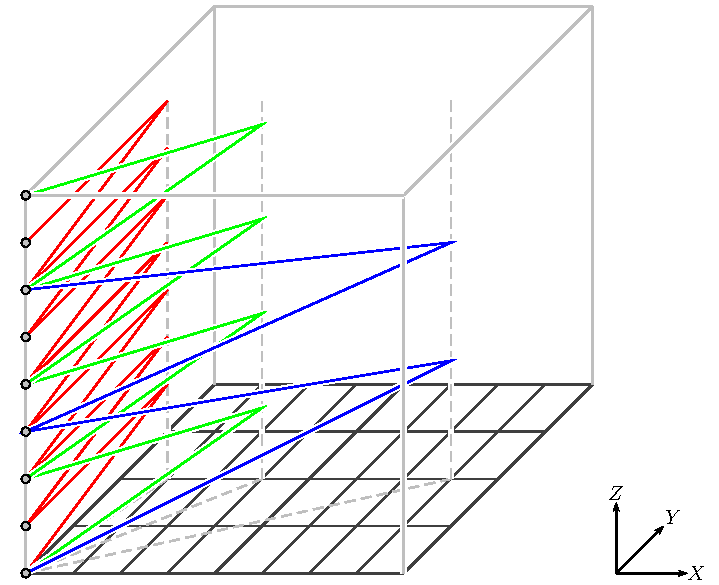
\includegraphics{CutwidthConstruction}}{Construction
of collinear $1$-bend drawing in \lemref{CutwidthUpperBound}.}

The constants in  \lemref{CutwidthUpperBound} can be tweaked as follows.

\begin{lemma}
\lemlabel{CutwidthUpperBoundSmall} 
Let $G$ be a graph with $n$ vertices and cutwidth $c$.
Then $G$ has a $1$-bend collinear  $3\times\ceil{(c-2)/2}\times n$
drawing. The volume is at most $3(c-1)n/2$.
\end{lemma}

%S = \{(-1,0),(1,0)\} \cup \{(x,y) : y\in\{-1,1\}, -1\le x\le 
%\ceil(c-6)/2\rceil\}

\begin{proof} Let $S=\{(-1,0),(1,0)\}\cup\{(x,y):y\in\{-1,1\},-1\leq x\leq
\ceil{(c-6)/2}\}$. Then $S$ consists of at least $c$ gridpoints that  are
visible from the origin.  The result follows from the proof of
\lemref{CutwidthUpperBound}. \end{proof}

Since the cutwidth of $K_n$ is $n^2/4$ we have:

\begin{corollary}
\corlabel{CollinearCompleteGraph} 
The minimum volume for a $1$-bend collinear drawing of the complete graph $K_n$ 
is $\Theta(n^3)$. For all $X\geq1$, $K_n$  has a $1$-bend collinear 
$X\times\Oh{n^2/X}\times n$ drawing with the vertices on the $Z$-axis.
Furthermore, $K_n$ has a $1$-bend collinear  
$3\times\ceil{n^2/8}\times n$ drawing with volume at most $3n^3/8$.\qed
\end{corollary}

%%%%%%%%%%%%%%%%%%%%%%%%%%%%%%%%%%%%%%%%%%%%%%%%%%%%%%%%%%%%%%%%%%%%%%%
\mySection{Proof of \thmref{Main}}{Main}
%%%%%%%%%%%%%%%%%%%%%%%%%%%%%%%%%%%%%%%%%%%%%%%%%%%%%%%%%%%%%%%%%%%%%%%%%%%%%%

Let $P=\ceil{\half\log_4n}$ and $Q=\ceil{n/P}$. Let $V(K_n)= \{ v_{a,i} : 1\leq
a\leq P, 1\leq i\leq Q\}$. Position each vertex $v_{a,i}$ at 
\begin{equation*}
(2a,\,aQ+i,\,0)\enspace.
\end{equation*}
For each $1\leq a\leq P$, the set of vertices $\{v_{a,i}:1\leq i\leq Q\}$
induces a complete graph $K_Q$, which is drawn 
using \corref{CollinearCompleteGraph} (with the dimensions permuted) 
in  the box
\begin{equation*}
[2a,2a+P]\times[aQ+1,(a+1)Q]\times[0,-c\,Q^2/P]\enspace,
\end{equation*}
for some constant $c$. For all $1\leq a<b\leq P$,  orient each edge
$e=(v_{a,i},v_{b,j})$,  and position the bend for $e$ at 
\begin{equation*}
r_e\;=\;(2a+1,\,bQ+j,\,4^{P-a}\, Q-i)\enspace,
\end{equation*}
as illustrated in \figref{VertexLayout}. We say $v_{a,i}r_e$ is an
\emph{outgoing} segment at $v_{a,i}$, and $r_ev_{b,j}$ is an \emph{incoming}
segment at $v_{b,j}$.

\Figure{VertexLayout}{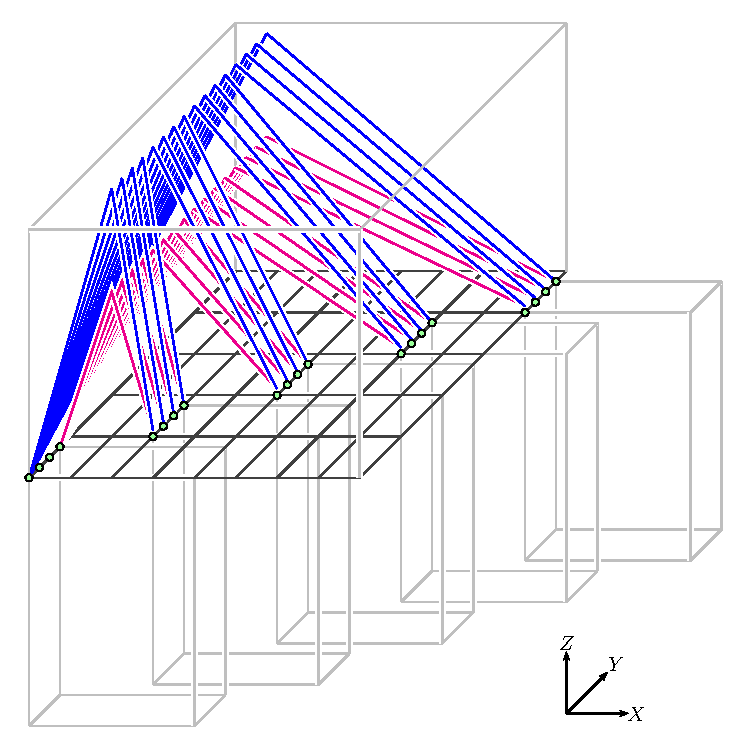
\includegraphics{VertexLayout}}{Construction of $1$-bend
drawing of $K_n$ in \thmref{Main}.}

Thus the bounding box is $\Oh{P}\times\Oh{n}\times\Oh{4^PQ+Q^2/P}$, which is 
$\Oh{\log n}\times\Oh{n}\times\Oh{n^{3/2}/\log n\,+\,n^2/\log^3n}$, which is
$\Oh{\log n}\times\Oh{n}\times\Oh{n^2/\log^3n}$. Hence the volume is
\Oh{n^3/\log^2n}. It remains to prove that there are no edge crossings. By 
\corref{CollinearCompleteGraph} all edges below the $Z=0$ plane do not cross.
We now only consider edges above the $Z=0$ plane. 

Each point in an outgoing segment at $v_{a,i}$ has an $X$-coordinate in
$[2a,2a+1]$. Thus an outgoing segment at some vertex $v_{a_1,i_1}$ does not
intersect an outgoing segment at some vertex $v_{a_2,i_2}$ whenever $a_1\ne
a_2$. Clearly an outgoing segment at $v_{a,i_1}$ is not coplanar with an
outgoing segment at $v_{a,i_2}$ whenever $i_1\ne i_2$, and thus these segments
do not cross. Since each bend is assigned a unique gridpoint, any two outgoing
segments at the same vertex $v_{a,i}$ do not cross. Thus no two outgoing
segments cross.

Each point in an incoming segment at $v_{b,j}$ has a $Y$-coordinate of $bQ+j$.
Thus incoming segments at distinct vertices do not cross.  Since each bend is
assigned a unique gridpoint, any two incoming segments at the same vertex do not
cross. Thus no two incoming segments cross.

To prove that an incoming segment does not cross an outgoing segment, we claim
that in the projection of the edges on the $Y=0$ plane,  an incoming segment
does not cross an outgoing segment. In the remainder of the proof we work
solely in the $Y=0$ plane, and use $(X,Z)$ coordinates.

The projection in the $Y=0$ plane 
of an outgoing segment at a vertex $v_{a,i}$  is the segment 
\begin{equation*}
s_1=(2a,0)\rightarrow(2a+1,4^{P-a}\,Q-i)\enspace.
\end{equation*}
The projection in the $Y=0$ plane of the incoming segment of an edge
$(v_{c,k},v_{d,\ell})$  is the segment
\begin{equation*}
s_2=(2c+1,4^{P-c}\,Q-k)\rightarrow(2d,0).
\end{equation*}

For there to be a crossing clearly we must have $c<a<d$. To prove that there is
no crossing it suffices to show that the $Z$-coordinate of $s_2$ is greater
than the $Z$-coordinate of $s_1$ when $X=2a+1$.
Now $s_2$ is contained in the line 
\begin{equation*}
Z=\frac{4^{P-c}\,Q-k}{2c+1-2d}(X-2d)\enspace.
\end{equation*}
Thus the $Z$-coordinate of $s_2$ at $X=2a+1$ is at least
\begin{equation*}
\frac{4^{P-c}\,Q-Q}{2c+1-2d}(2a+1-2d)\enspace.
\end{equation*}
Thus it suffices to prove that 
\begin{equation}
\eqnlabel{SomeEqn}
\frac{4^{P-c}\,Q-Q}{2c+1-2d}(2a+1-2d)\;>\;4^{P-a}\,Q\enspace.
\end{equation}
Clearly \eqnref{SomeEqn} is implied if it is proved with $a=c+1$ and $d=c+2$.
In this case, \eqnref{SomeEqn} reduces to
\begin{equation*}
\frac{4^{P-c}-1}{3}\;>\;4^{P-c-1}\enspace.
\end{equation*}
That is,
$4^{P-c-1}>1$,
which is true since $c\leq P-2$.
This completes the proof.

%%%%%%%%%%%%%%%%%%%%%%%%%%%%%%%%%%%%%%%%%%%%%%%%%%%%%%%%%%%%%%%%%%%%%%%%%%%%%%%%
\bibliographystyle{myBibliographyStyle}
\bibliography{myBibliography,myConferences}
%%%%%%%%%%%%%%%%%%%%%%%%%%%%%%%%%%%%%%%%%%%%%%%%%%%%%%%%%%%%%%%%%%%%%%%%%%%%%%%%

\end{document}

